% Options for packages loaded elsewhere
\PassOptionsToPackage{unicode}{hyperref}
\PassOptionsToPackage{hyphens}{url}
%
\documentclass[
]{article}
\usepackage{lmodern}
\usepackage{amsmath}
\usepackage{ifxetex,ifluatex}
\ifnum 0\ifxetex 1\fi\ifluatex 1\fi=0 % if pdftex
  \usepackage[T1]{fontenc}
  \usepackage[utf8]{inputenc}
  \usepackage{textcomp} % provide euro and other symbols
  \usepackage{amssymb}
\else % if luatex or xetex
  \usepackage{unicode-math}
  \defaultfontfeatures{Scale=MatchLowercase}
  \defaultfontfeatures[\rmfamily]{Ligatures=TeX,Scale=1}
\fi
% Use upquote if available, for straight quotes in verbatim environments
\IfFileExists{upquote.sty}{\usepackage{upquote}}{}
\IfFileExists{microtype.sty}{% use microtype if available
  \usepackage[]{microtype}
  \UseMicrotypeSet[protrusion]{basicmath} % disable protrusion for tt fonts
}{}
\makeatletter
\@ifundefined{KOMAClassName}{% if non-KOMA class
  \IfFileExists{parskip.sty}{%
    \usepackage{parskip}
  }{% else
    \setlength{\parindent}{0pt}
    \setlength{\parskip}{6pt plus 2pt minus 1pt}}
}{% if KOMA class
  \KOMAoptions{parskip=half}}
\makeatother
\usepackage{xcolor}
\IfFileExists{xurl.sty}{\usepackage{xurl}}{} % add URL line breaks if available
\IfFileExists{bookmark.sty}{\usepackage{bookmark}}{\usepackage{hyperref}}
\hypersetup{
  pdftitle={Afleverin 2},
  hidelinks,
  pdfcreator={LaTeX via pandoc}}
\urlstyle{same} % disable monospaced font for URLs
\usepackage[margin=1in]{geometry}
\usepackage{color}
\usepackage{fancyvrb}
\newcommand{\VerbBar}{|}
\newcommand{\VERB}{\Verb[commandchars=\\\{\}]}
\DefineVerbatimEnvironment{Highlighting}{Verbatim}{commandchars=\\\{\}}
% Add ',fontsize=\small' for more characters per line
\usepackage{framed}
\definecolor{shadecolor}{RGB}{248,248,248}
\newenvironment{Shaded}{\begin{snugshade}}{\end{snugshade}}
\newcommand{\AlertTok}[1]{\textcolor[rgb]{0.94,0.16,0.16}{#1}}
\newcommand{\AnnotationTok}[1]{\textcolor[rgb]{0.56,0.35,0.01}{\textbf{\textit{#1}}}}
\newcommand{\AttributeTok}[1]{\textcolor[rgb]{0.77,0.63,0.00}{#1}}
\newcommand{\BaseNTok}[1]{\textcolor[rgb]{0.00,0.00,0.81}{#1}}
\newcommand{\BuiltInTok}[1]{#1}
\newcommand{\CharTok}[1]{\textcolor[rgb]{0.31,0.60,0.02}{#1}}
\newcommand{\CommentTok}[1]{\textcolor[rgb]{0.56,0.35,0.01}{\textit{#1}}}
\newcommand{\CommentVarTok}[1]{\textcolor[rgb]{0.56,0.35,0.01}{\textbf{\textit{#1}}}}
\newcommand{\ConstantTok}[1]{\textcolor[rgb]{0.00,0.00,0.00}{#1}}
\newcommand{\ControlFlowTok}[1]{\textcolor[rgb]{0.13,0.29,0.53}{\textbf{#1}}}
\newcommand{\DataTypeTok}[1]{\textcolor[rgb]{0.13,0.29,0.53}{#1}}
\newcommand{\DecValTok}[1]{\textcolor[rgb]{0.00,0.00,0.81}{#1}}
\newcommand{\DocumentationTok}[1]{\textcolor[rgb]{0.56,0.35,0.01}{\textbf{\textit{#1}}}}
\newcommand{\ErrorTok}[1]{\textcolor[rgb]{0.64,0.00,0.00}{\textbf{#1}}}
\newcommand{\ExtensionTok}[1]{#1}
\newcommand{\FloatTok}[1]{\textcolor[rgb]{0.00,0.00,0.81}{#1}}
\newcommand{\FunctionTok}[1]{\textcolor[rgb]{0.00,0.00,0.00}{#1}}
\newcommand{\ImportTok}[1]{#1}
\newcommand{\InformationTok}[1]{\textcolor[rgb]{0.56,0.35,0.01}{\textbf{\textit{#1}}}}
\newcommand{\KeywordTok}[1]{\textcolor[rgb]{0.13,0.29,0.53}{\textbf{#1}}}
\newcommand{\NormalTok}[1]{#1}
\newcommand{\OperatorTok}[1]{\textcolor[rgb]{0.81,0.36,0.00}{\textbf{#1}}}
\newcommand{\OtherTok}[1]{\textcolor[rgb]{0.56,0.35,0.01}{#1}}
\newcommand{\PreprocessorTok}[1]{\textcolor[rgb]{0.56,0.35,0.01}{\textit{#1}}}
\newcommand{\RegionMarkerTok}[1]{#1}
\newcommand{\SpecialCharTok}[1]{\textcolor[rgb]{0.00,0.00,0.00}{#1}}
\newcommand{\SpecialStringTok}[1]{\textcolor[rgb]{0.31,0.60,0.02}{#1}}
\newcommand{\StringTok}[1]{\textcolor[rgb]{0.31,0.60,0.02}{#1}}
\newcommand{\VariableTok}[1]{\textcolor[rgb]{0.00,0.00,0.00}{#1}}
\newcommand{\VerbatimStringTok}[1]{\textcolor[rgb]{0.31,0.60,0.02}{#1}}
\newcommand{\WarningTok}[1]{\textcolor[rgb]{0.56,0.35,0.01}{\textbf{\textit{#1}}}}
\usepackage{graphicx}
\makeatletter
\def\maxwidth{\ifdim\Gin@nat@width>\linewidth\linewidth\else\Gin@nat@width\fi}
\def\maxheight{\ifdim\Gin@nat@height>\textheight\textheight\else\Gin@nat@height\fi}
\makeatother
% Scale images if necessary, so that they will not overflow the page
% margins by default, and it is still possible to overwrite the defaults
% using explicit options in \includegraphics[width, height, ...]{}
\setkeys{Gin}{width=\maxwidth,height=\maxheight,keepaspectratio}
% Set default figure placement to htbp
\makeatletter
\def\fps@figure{htbp}
\makeatother
\setlength{\emergencystretch}{3em} % prevent overfull lines
\providecommand{\tightlist}{%
  \setlength{\itemsep}{0pt}\setlength{\parskip}{0pt}}
\setcounter{secnumdepth}{-\maxdimen} % remove section numbering
\ifluatex
  \usepackage{selnolig}  % disable illegal ligatures
\fi

\title{Afleverin 2}
\author{}
\date{\vspace{-2.5em}}

\begin{document}
\maketitle

Vi har givet et signal

\[
y(x)= 9 sin(x)-2sin(5x)
\]

\hypertarget{a-lav-en-python-plot-af-funktionen-foroven-med-n-100-juxe6vnt-fordelt-over-intervallet-0-6.}{%
\subsection{a) Lav en python plot af funktionen foroven med n = 100
jævnt fordelt over intervallet {[}0,
6{]}.}\label{a-lav-en-python-plot-af-funktionen-foroven-med-n-100-juxe6vnt-fordelt-over-intervallet-0-6.}}

\begin{Shaded}
\begin{Highlighting}[]
\ImportTok{import}\NormalTok{ matplotlib.pyplot }\ImportTok{as}\NormalTok{ plt}
\ImportTok{import}\NormalTok{ numpy }\ImportTok{as}\NormalTok{ np}
\end{Highlighting}
\end{Shaded}

Til at lave plottet af den ovenstående funktino benytter jeg mig af
modulet \texttt{matplotlib}.

\begin{Shaded}
\begin{Highlighting}[]
\NormalTok{x }\OperatorTok{=}\NormalTok{ np.linspace(}\DecValTok{0}\NormalTok{, }\DecValTok{6}\NormalTok{, }\DecValTok{100}\NormalTok{)}
\NormalTok{y }\OperatorTok{=} \DecValTok{9} \OperatorTok{*}\NormalTok{ np.sin(x) }\OperatorTok{{-}} \DecValTok{2} \OperatorTok{*}\NormalTok{ np.sin(}\DecValTok{5}\OperatorTok{*}\NormalTok{x)}
\NormalTok{fig, ax }\OperatorTok{=}\NormalTok{ plt.subplots()}
\NormalTok{ax.set\_aspect(}\StringTok{"equal"}\NormalTok{)}
\NormalTok{ax.plot(x, y)}
\NormalTok{plt.show()}
\end{Highlighting}
\end{Shaded}

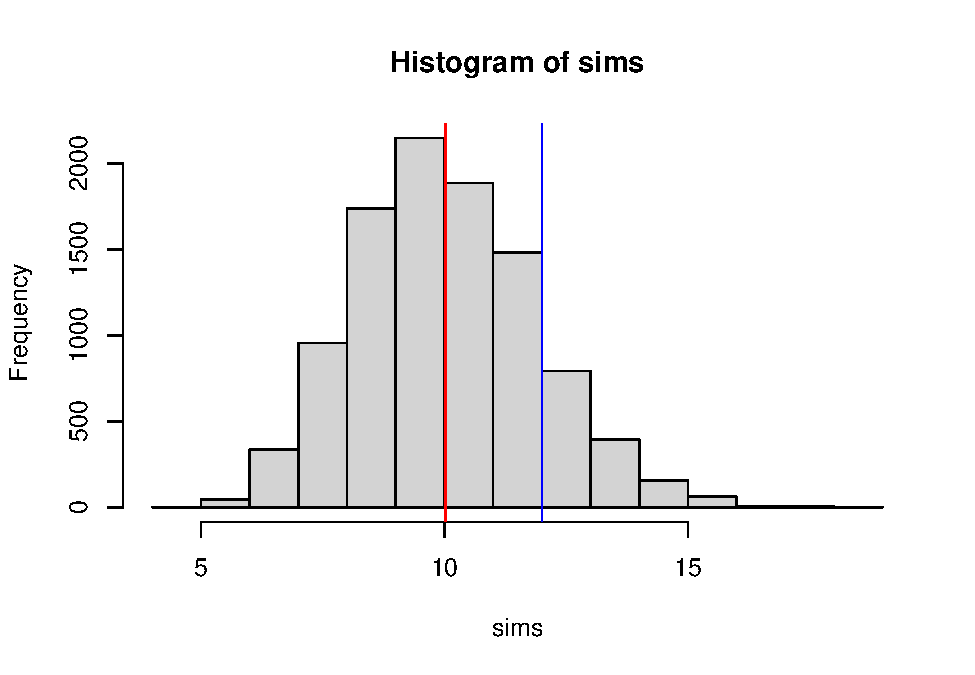
\includegraphics{aflevering-2_files/figure-latex/unnamed-chunk-2-1.pdf}

\hypertarget{b-tilfuxf8j-stuxf8j-til-funktionen-og-plot-det.}{%
\subsection{b) Tilføj støj til funktionen og plot
det.}\label{b-tilfuxf8j-stuxf8j-til-funktionen-og-plot-det.}}

Her skal vi i y formlen tilføje følgende:

\[
y_{støj} = y + rng.standardnormal(n)
\]

\begin{Shaded}
\begin{Highlighting}[]
\NormalTok{n }\OperatorTok{=} \DecValTok{100}
\NormalTok{rng }\OperatorTok{=}\NormalTok{ np.random.default\_rng()}
\NormalTok{støj }\OperatorTok{=}\NormalTok{ rng.standard\_normal(n)}
\end{Highlighting}
\end{Shaded}

\begin{Shaded}
\begin{Highlighting}[]
\NormalTok{y\_støj }\OperatorTok{=}\NormalTok{ y }\OperatorTok{+}\NormalTok{ støj}
\NormalTok{fig, ax }\OperatorTok{=}\NormalTok{ plt.subplots()}
\NormalTok{ax.set\_aspect(}\StringTok{"equal"}\NormalTok{)}
\NormalTok{ax.plot(x, y\_støj)}
\NormalTok{plt.show()}
\end{Highlighting}
\end{Shaded}

\includegraphics{aflevering-2_files/figure-latex/unnamed-chunk-4-1.pdf}

\hypertarget{c}{%
\subsection{c)}\label{c}}

Givet en vektor v og et heltal offset vil funktionen np.diag(v, offset)
danne en matrix med v langs en skrå linje hvor start punktet er forskudt
fra det øverste venstre hjørne med offset. Brug np.diag, eventuelt
kombineret med np.ones(), tre gange til at konstruere matricen 𝐴 ∈ ℝ𝑛×𝑛
der har formen

\begin{Shaded}
\begin{Highlighting}[]
\ControlFlowTok{for}\NormalTok{ n }\KeywordTok{in} \BuiltInTok{range}\NormalTok{(}\DecValTok{1}\NormalTok{,}\DecValTok{101}\NormalTok{):}
\NormalTok{  v }\OperatorTok{=} \DecValTok{1}\OperatorTok{/}\DecValTok{3} \OperatorTok{*}\NormalTok{ np.ones((}\DecValTok{1}\NormalTok{, n))}
\NormalTok{  A1 }\OperatorTok{=}\NormalTok{ np.diag(v[}\DecValTok{0}\NormalTok{], }\OperatorTok{{-}}\DecValTok{1}\NormalTok{) }
\NormalTok{  A2 }\OperatorTok{=}\NormalTok{ np.diag(v[}\DecValTok{0}\NormalTok{], }\DecValTok{0}\NormalTok{)}
\NormalTok{  A3 }\OperatorTok{=}\NormalTok{  np.diag(v[}\DecValTok{0}\NormalTok{], }\DecValTok{1}\NormalTok{)}
\NormalTok{  A }\OperatorTok{=}\NormalTok{ A1[}\DecValTok{0}\NormalTok{:n, }\DecValTok{0}\NormalTok{:n] }\OperatorTok{+}\NormalTok{ A2[}\DecValTok{0}\NormalTok{:n, }\DecValTok{0}\NormalTok{:n] }\OperatorTok{+}\NormalTok{ A3[}\DecValTok{0}\NormalTok{:n, }\DecValTok{0}\NormalTok{:n]}
\end{Highlighting}
\end{Shaded}

Foroven har jeg forsøgt a kontruer den ønskede matrice.

\hypertarget{d-plot-aystuxf8j.-her-skal-vi-se-om-den-har-en-form-der-mindere-mere-om-y-end}{%
\subsection{d) Plot Aystøj. Her skal vi se om den har en form der
mindere mere om y
end}\label{d-plot-aystuxf8j.-her-skal-vi-se-om-den-har-en-form-der-mindere-mere-om-y-end}}

på ystøj.

\begin{Shaded}
\begin{Highlighting}[]
\NormalTok{A\_y\_støj }\OperatorTok{=}\NormalTok{ A}\OperatorTok{*}\NormalTok{y }\OperatorTok{+}\NormalTok{ støj}
\NormalTok{fig, ax }\OperatorTok{=}\NormalTok{ plt.subplots()}
\NormalTok{ax.set\_aspect(}\StringTok{"equal"}\NormalTok{)}
\NormalTok{ax.plot(x, A\_y\_støj)}
\end{Highlighting}
\end{Shaded}

\begin{verbatim}
## [<matplotlib.lines.Line2D object at 0x7faec7312e80>, <matplotlib.lines.Line2D object at 0x7faec7312e20>, <matplotlib.lines.Line2D object at 0x7faec7312c70>, <matplotlib.lines.Line2D object at 0x7faec7312c40>, <matplotlib.lines.Line2D object at 0x7faec7312fa0>, <matplotlib.lines.Line2D object at 0x7faec73200a0>, <matplotlib.lines.Line2D object at 0x7faec7320160>, <matplotlib.lines.Line2D object at 0x7faec7320220>, <matplotlib.lines.Line2D object at 0x7faec73202e0>, <matplotlib.lines.Line2D object at 0x7faec73203a0>, <matplotlib.lines.Line2D object at 0x7faec71b3fa0>, <matplotlib.lines.Line2D object at 0x7faec7320460>, <matplotlib.lines.Line2D object at 0x7faec73205b0>, <matplotlib.lines.Line2D object at 0x7faec7320670>, <matplotlib.lines.Line2D object at 0x7faec7320730>, <matplotlib.lines.Line2D object at 0x7faec73207f0>, <matplotlib.lines.Line2D object at 0x7faec73208b0>, <matplotlib.lines.Line2D object at 0x7faec7320970>, <matplotlib.lines.Line2D object at 0x7faec7320a30>, <matplotlib.lines.Line2D object at 0x7faec7320af0>, <matplotlib.lines.Line2D object at 0x7faec7320bb0>, <matplotlib.lines.Line2D object at 0x7faec7320c70>, <matplotlib.lines.Line2D object at 0x7faec7320d30>, <matplotlib.lines.Line2D object at 0x7faec7320df0>, <matplotlib.lines.Line2D object at 0x7faec7320eb0>, <matplotlib.lines.Line2D object at 0x7faec7320f70>, <matplotlib.lines.Line2D object at 0x7faec7327070>, <matplotlib.lines.Line2D object at 0x7faec7327130>, <matplotlib.lines.Line2D object at 0x7faec73271f0>, <matplotlib.lines.Line2D object at 0x7faec73272b0>, <matplotlib.lines.Line2D object at 0x7faec7327370>, <matplotlib.lines.Line2D object at 0x7faec7327430>, <matplotlib.lines.Line2D object at 0x7faec73274f0>, <matplotlib.lines.Line2D object at 0x7faec73275e0>, <matplotlib.lines.Line2D object at 0x7faec73276a0>, <matplotlib.lines.Line2D object at 0x7faec7327760>, <matplotlib.lines.Line2D object at 0x7faec7327820>, <matplotlib.lines.Line2D object at 0x7faec73278e0>, <matplotlib.lines.Line2D object at 0x7faec73279a0>, <matplotlib.lines.Line2D object at 0x7faec7327a60>, <matplotlib.lines.Line2D object at 0x7faec7327b20>, <matplotlib.lines.Line2D object at 0x7faec7327be0>, <matplotlib.lines.Line2D object at 0x7faec7327ca0>, <matplotlib.lines.Line2D object at 0x7faec7327d60>, <matplotlib.lines.Line2D object at 0x7faec7327e20>, <matplotlib.lines.Line2D object at 0x7faec7327ee0>, <matplotlib.lines.Line2D object at 0x7faec7327fa0>, <matplotlib.lines.Line2D object at 0x7faec732e0a0>, <matplotlib.lines.Line2D object at 0x7faec732e160>, <matplotlib.lines.Line2D object at 0x7faec732e220>, <matplotlib.lines.Line2D object at 0x7faec732e2e0>, <matplotlib.lines.Line2D object at 0x7faec732e3a0>, <matplotlib.lines.Line2D object at 0x7faec732e460>, <matplotlib.lines.Line2D object at 0x7faec732e520>, <matplotlib.lines.Line2D object at 0x7faec732e5e0>, <matplotlib.lines.Line2D object at 0x7faec732e6a0>, <matplotlib.lines.Line2D object at 0x7faec732e760>, <matplotlib.lines.Line2D object at 0x7faec732e820>, <matplotlib.lines.Line2D object at 0x7faec732e8e0>, <matplotlib.lines.Line2D object at 0x7faec732e9a0>, <matplotlib.lines.Line2D object at 0x7faec732ea60>, <matplotlib.lines.Line2D object at 0x7faec732eb20>, <matplotlib.lines.Line2D object at 0x7faec732ebe0>, <matplotlib.lines.Line2D object at 0x7faec732eca0>, <matplotlib.lines.Line2D object at 0x7faec732ed60>, <matplotlib.lines.Line2D object at 0x7faec732ee20>, <matplotlib.lines.Line2D object at 0x7faec732eee0>, <matplotlib.lines.Line2D object at 0x7faec732efa0>, <matplotlib.lines.Line2D object at 0x7faec73350a0>, <matplotlib.lines.Line2D object at 0x7faec7335160>, <matplotlib.lines.Line2D object at 0x7faec7335220>, <matplotlib.lines.Line2D object at 0x7faec73352e0>, <matplotlib.lines.Line2D object at 0x7faec73353a0>, <matplotlib.lines.Line2D object at 0x7faec7335460>, <matplotlib.lines.Line2D object at 0x7faec7335520>, <matplotlib.lines.Line2D object at 0x7faec73355e0>, <matplotlib.lines.Line2D object at 0x7faec73356a0>, <matplotlib.lines.Line2D object at 0x7faec7335760>, <matplotlib.lines.Line2D object at 0x7faec7335820>, <matplotlib.lines.Line2D object at 0x7faec73358e0>, <matplotlib.lines.Line2D object at 0x7faec73359a0>, <matplotlib.lines.Line2D object at 0x7faec7335a60>, <matplotlib.lines.Line2D object at 0x7faec7335b20>, <matplotlib.lines.Line2D object at 0x7faec7335be0>, <matplotlib.lines.Line2D object at 0x7faec7335ca0>, <matplotlib.lines.Line2D object at 0x7faec7335d60>, <matplotlib.lines.Line2D object at 0x7faec7335e20>, <matplotlib.lines.Line2D object at 0x7faec7335ee0>, <matplotlib.lines.Line2D object at 0x7faec7335fa0>, <matplotlib.lines.Line2D object at 0x7faec733b0a0>, <matplotlib.lines.Line2D object at 0x7faec733b160>, <matplotlib.lines.Line2D object at 0x7faec733b220>, <matplotlib.lines.Line2D object at 0x7faec733b2e0>, <matplotlib.lines.Line2D object at 0x7faec733b3a0>, <matplotlib.lines.Line2D object at 0x7faec733b460>, <matplotlib.lines.Line2D object at 0x7faec733b520>, <matplotlib.lines.Line2D object at 0x7faec733b5e0>, <matplotlib.lines.Line2D object at 0x7faec733b6a0>, <matplotlib.lines.Line2D object at 0x7faec733b760>, <matplotlib.lines.Line2D object at 0x7faec733b820>]
\end{verbatim}

\begin{Shaded}
\begin{Highlighting}[]
\NormalTok{plt.show()}
\end{Highlighting}
\end{Shaded}

\includegraphics{aflevering-2_files/figure-latex/unnamed-chunk-6-1.pdf}

Der er noget som gør galt i min plot. Jeg tror det skyldes at jeg ikke
får splitte min matrice A op i en enkelt array, så nu ser den som en
nested funktion.

Dog med antagelse af jeg fik et plot, som minder mere om det
oprindelige, så vil det ligne mere da vi inkludere flere multiplikation
af nul, som gør at vi fjerne noget støj.

\hypertarget{e-uxe6ndre-puxe5-vuxe6gtning-i-a-og-lave-en-matrix-b-som-er-bedre-end-a.}{%
\subsection{e) Ændre på vægtning i A og lave en matrix B, som er bedre
end
A.}\label{e-uxe6ndre-puxe5-vuxe6gtning-i-a-og-lave-en-matrix-b-som-er-bedre-end-a.}}

Jeg vil ikke kaste mig ud i denne da jeg ikke komme til at ramme plet i
forhold til at kunne lave et plot.

Men selvfølgelig kan vi reducerer mere støj ved at lave en mere optimal
vægtning ved at inkluderer en Matrix B.

\begin{quote}
Husk at gå igang lidt før, så du kan afklare tvivl sprøgsmål.
\end{quote}

\end{document}
